\documentclass[12pt,a4paper,oneside,article]{memoir}

\usepackage{polyglossia}
\setdefaultlanguage{english}
\usepackage{fontspec}

\defaultfontfeatures{Ligatures=TeX}
\newfontfeature{Microtype}{protrusion=default;expansion=default}
\usepackage[final]{microtype}
\setmainfont{Linux Libertine O}
\setsansfont{Linux Biolinum O}
\setmonofont{DejaVu Sans Mono}

\usepackage{subfiles}
\usepackage{tabularx}
\usepackage{tabu}
\usepackage{booktabs}
\usepackage{multirow}
\usepackage{float}
\usepackage{amsmath,amsfonts,amssymb}
\usepackage{mathtools}
\usepackage[shortlabels]{enumitem}

\usepackage{tikz}
\usepackage[subpreambles=true]{standalone}
\usepackage{import}
\usepackage{graphicx}
\usepackage{hyperref}
\hypersetup{hidelinks}
\usepackage{xcolor, colortbl, array}

\usepackage{listings}
\usepackage{color}
\lstset{
  language=Python,
  frame=tb,
  breaklines=true,
  breakatwhitespace=true,
  keepspaces=true,
  columns=fullflexible,
  showspaces=false,
  showstringspaces=false,
  showtabs=false,
  basicstyle=\ttfamily\footnotesize
}

\usepackage[autostyle,strict,autopunct]{csquotes}
\usepackage[style=ieee,backend=biber]{biblatex}
\bibliography{bibliography}

\usepackage{chngcntr}
\counterwithin{table}{section}
\numberwithin{equation}{chapter}
\counterwithin{figure}{section}
\setenumerate[0]{label= (\alph*)}
\AtBeginDocument{\counterwithin{lstlisting}{section}}
\counterwithout{section}{chapter}
\newsubfloat{figure}

\chapterstyle{article}
\pagestyle{headings}

\title{MOCCA Operational Controller for Coffee Availability}
\author{Eivind Dagsland Halderaker \and Sondre Åsemoen Nilsen}
\date{INF219, Spring 2019}
\begin{document}
\begin{titlingpage}

\newcommand{\HRule}{\rule{\linewidth}{0.5mm}}
\centering

\textsc{\LARGE University of Bergen \\ Department of informatics}\\[1.5cm] %

\HRule\\[0.5cm]
\begin{Huge}
	\bfseries{\thetitle}\\[0.7cm]
\end{Huge}
\HRule\\[0.5cm]

{\large \theauthor}\\
{\large \emph{Supervisor:} Albin Severinson\\[2cm]}

\centerline{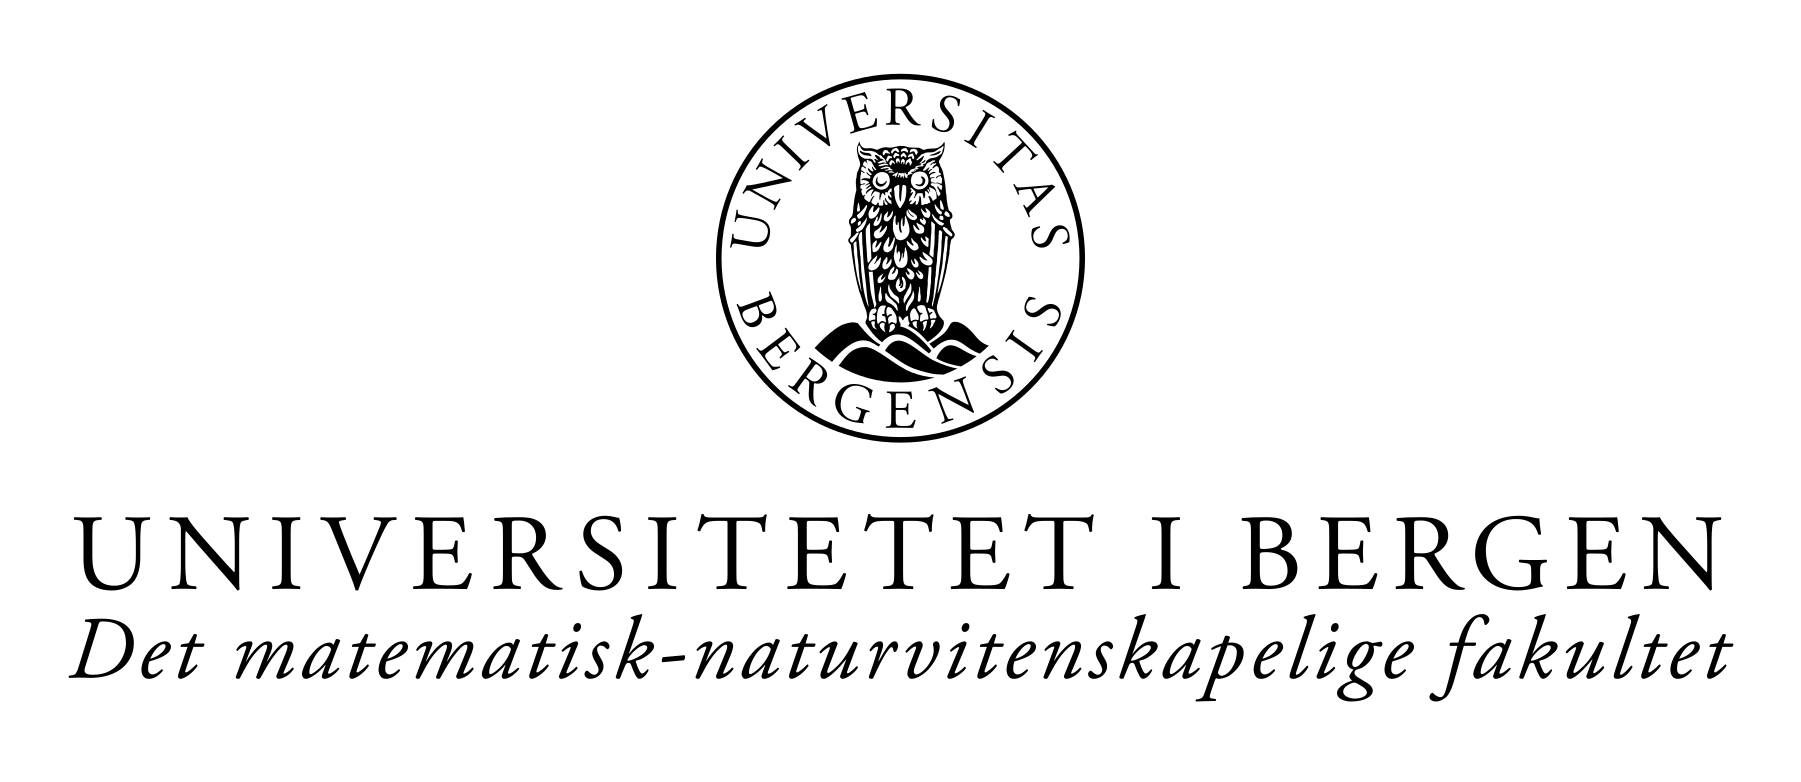
\includegraphics[scale=1.9]{figures/canvasWithFaculty}}
{\large \thedate}\\[3cm]
\vfill

\begin{abstract}
One of the challenges facing students at the informatics department at the 
University of Bergen is knowing whether there is fresh coffee available in the 
study hall or not.  Students often lose valuable study time by walking over to 
the coffee maker, only to discover that the pot is empty or that the coffee is 
cold. In this report, we present \textit{MOCCA} (MOCCA Operational Controller 
for Coffee Availability), an Internet of Things coffee brewer designed to 
address this issue. Specifically, \textit{MOCCA} enables students to visit a 
website and immediately know the amount of remaining coffee, its temperature, 
and its age.
\end{abstract}
\end{titlingpage}

\clearpage

\section{Introduction}\label{sec:introduction}
At our study hall our most prized possession is probably the drip coffee
machine. It is a valuable piece of comfort that we have, and is used from early
in the morning until the last student goes home. The problem is that you can
never be sure when there is coffee, and whenever there is none left you waste
precious minutes in the couch waiting for it to finish brewing. There have been
many attempts at solving this problem throughout the years, none of which have
survived past the initial testing phase. This project breaks the chain and have
a working product that can withstand the test of time.

In this report, we present \textit{MOCCA}: MOCCA Operational Controller for
Coffee Availability, a system for measuring both the temperature, age, and
quantity of coffee. It orchestrates a REST API, which is a stateless web service
that allows clients to make HTTP requests to a server via specific URLs. If a
request is valid, the server then sends a response back containing the requested
data, and if the request did not succeed information about why not. Our API
gives information about the temperature of the coffee, how old the brew is, and
an estimate of the amount of coffee remaining. In turn this API is then used to
display this information on a website.

\textit{MOCCA} achieves this by combining a contact-less infrared temperature
sensor and an electrical current sensor connected to an Arduino Uno and a camera
connected to a Raspberry Pi, which also doubles as our data cruncher. Measuring
temperature is fairly straight-forward with an infrared sensor. However,
figuring out how old a brew is is a bit trickier. To measure the age of a brew
we monitor the amount of current the brewer is drawing. A coffee brewer has
essentially three states: turned off, brewing, and warming. By saving time
stamps at the start of a new brew, it is trivial to calculate age at a given
point. Quantity is measured by image processing. Images are taken of the coffee
pot and we estimate the amount of coffee remaining by counting the number of
dark pixels,while accounting for the background of the pot.

This approach has the benefit of giving the students near our study hall 
real-time information about the drip brewer. Students are still able to use the 
brewer as usual without any interference from our product. A hard requirement
is that the machine has to be non-intrusive, we cannot interfere or take apart
the brewer, not can we sacrifice the ease of access and use for it.

The remainder of the report is organized as follows. Section
\ref{sec:system-overview} is an overview as well as a technical description of
the system and its various subsystems. In Section \ref{sec:conclusion}, we give
our concluding remarks. Finally in Section \ref{sec:future-work}, and ending
with acknowledgements in section \ref{sec:acknowledgements}.

\section{System overview}\label{sec:system-overview}
\begin{figure}[h]
  \centerfloat{}
  \scalebox{.75}{\documentclass[border=3mm]{standalone}
\usepackage{tikz}
\usetikzlibrary{positioning,fit,arrows.meta,backgrounds}

\tikzset{
  module/.style={%
    draw, rounded corners,
    minimum width=#1,
    minimum height=7mm,
    font=\sffamily
  },
  module/.default=2cm,
  container/.style={
    draw, rounded corners,
    minimum-width=#1,
    minimum height=5cm,
    font=\sffamily
  },
  container/.default=2cm,
  small/.style={
    draw, rounded corners,
    minimum height=2.5cm
    font=\sffamily
  },
  >=LaTeX
}

\begin{document}
\begin{tikzpicture}[->]
  % Arduino box
  \node[module] (Read) {Read from sensors};
  \node[module, below left=1cm and -1cm of Read] (Temp) {Temperature};
  \node[module, below right=1cm and -1cm of Read] (Power) {Power draw};
  \node[small,fit=(Read) (Temp) (Power), draw, label={Arduino}] (SensorBox) {};
  \draw[->] (Read)--(Temp);
  \draw[->] (Read)--(Power);
  % Raspberry Pi processing box
  \node[module, right=2cm of Read] (Camera) {Take picture};
  \node[module, below=of Camera] (CamProcess) {Process};
  \node[small, fit=(Camera) (CamProcess), draw, label={Raspberry Pi}] (Pi2Box) {};
  \draw[->] (Camera)--(CamProcess);
  % Data collection box
  \node[container, fit=(SensorBox) (Pi2Box) (Loop),
  draw, inner xsep=2mm, inner ysep=.5cm,
  label={Data collection}] (DataCollectionBox) {};

  % Data processing box
  \node[module, above right=-1.15cm and 2cm of DataCollectionBox] (AsyncLoop) {Async loop};
  \node[module, below=of AsyncLoop] (Data) {Data processing};
  \node[module, below=of Data] (Storage) {Storage};
  \node[container, fit={(AsyncLoop) (Data) (Storage)},
        draw, inner sep=2mm,
        label={Data processing}]
        (MainBox) {};
  \draw[->] (AsyncLoop)--(Data);
  \draw[->] (Data)--(Storage);

  % Connect main loop and async loop
  \draw[<->] (DataCollectionBox)--(MainBox);

  % Serve box
  \node[module, right=2cm of {AsyncLoop-|MainBox.east}] (Server) {Server};
  \node[module, below=of Server] (API) {API};
  \node[module, below=of API] (Website) {Website};
  \node[container, fit={(Server) (API) (Website)}, draw, inner sep=2mm, label={Serving}] (ServeBox) {};
  \draw[->] (Server)--(API);
  \path[] (Server) edge[bend left=52.5] node [left] {} (Website);
  \draw[->] (API)--(Website);
  \draw[->] (MainBox)--(ServeBox);
\end{tikzpicture}
\end{document}
%%% Local Variables:
%%% mode: latex
%%% TeX-master: t
%%% End:
}
  \caption{An overview of the system architecture for \textit{MOCCA}. There are
    two physically separate systems, an Arduino and a Raspberry Pi. The data
    collection subsystem uses both for taking a snapshot of the coffee at a
    given point in time. This data is passed to the data processing subsystems
    which transforms and stores this data, finally passing it on to the serving
    subsystem which serves this data to our API, and serves our website.
  }\label{fig:architecture}
\end{figure}
\textit{MOCCA} is composed of three subsystems that are responsible for
collecting sensor data, processing and storing this data and presenting the data
to the user, respectively. See figure \ref{fig:architecture}.

\subsection{Data collection}\label{sec:data-collection}
The first subsystem is the data collection system. It consists of an 
infrared sensor measuring the temperature of the coffee, a current sensor 
measuring current to determine the state of the brewer and a camera pointed 
towards the coffee for measuring amount of coffee. The two first sensors are 
controlled by the Arduino micro controller while the camera is connected to the 
Raspberry Pi.

\subsubsection{Arduino}\label{sec:arduino}
Our code on the Arduino runs in a loop, continuously reading from its sensors,
saving the data to a queue. This queue prevents the Raspberry Pi from reading
data in the middle of a write to the serial interface. The Arduino continuously
adds to the queue, discarding the last item in it for every reading, and waits
for the Raspberry Pi to send a predetermined message saying that it is ready for
data. Once the Arduino receives this message it enters a write-mode and fetches
the latest reading from the queue, returns it, clears the queue and exits the
current state returning to reading data.

\subsubsection{Raspberry Pi}\label{sec:raspberry-pi}
The Raspberry Pi 3+ is a small computer equipped with USB, HDMI, WiFi, and, most
important for us, support for a camera. Though lacking in computational power,
its size and affordability makes it a perfect data cruncher for our case as it
can fit in a compact container near the drip coffee brewer. We used the
Raspberry Pi Foundation's own camera accessory, which is plug-and-play while
still having more than high enough resolution. We only need a rough estimate of
how full the coffee pot is and high resolution means more data to be processed,
most of which is redundant.

\subsection{Data processing}\label{sec:data-processing}
The data processing subsystem is the core of our application. An asynchronous
task queue calls the data collection subsystem and once the data is collected
starts processing it. Every ten seconds an event fires which gathers the data
from the sensors and camera, and processes the data given. A lot of the heavy
lifting here is done in NumPy, a high-performance library for scientific
computing with Python. Once an image has been captured by our camera it is
transformed into a matrix of boolean values based on a threshold for brightness.
Thanks to the excellent performance given by NumPy, even the limited computing
power of the Raspberry Pi is no concern.

The temperature and power draw is simply read from the Arduino without any
processing necessary. This is not to say that we simply take the values and
insert them into our database, we still need to verify that the data that was
returned is valid data in our current state and what to do with it. There are a
number of moving parts, variables and possible states that we need to ensure are
all in sync and valid, requiring sophisticated error handling. How does the
subsystem know that the current state of the world is in order? As we are
processing data we need to determine if the data that was read and received
matches our current expected state and values, while also ensuring that the
possible causes of this does not cause the system to enter a state where no
further data will be valid. This is achieved by various safety checks and data
validation. Since the system runs on a ten second loop, our solution to invalid
data is to discard the current reading and wait for the next one.

For instance, the coffee machine can be powered off by two different parts: its
own power supply or the socket that it is connected to as both these run on
separate timers. This is simple enough, if there is no power going through the
current sensor we know that there's an outage and update the state of the brew
accordingly. If the temperature of the coffee is hotter than the brewer can
possibly achieve, we discard it. Or, if the temperature from the latest reading
to the one being processed is above our threshold for valid swings in
temperature, we discard it and wait for the next.

If our current assumed state is that the machine is keeping the coffee warm, a
reading where the temperature suddenly changes can for example be that someone
has taken away the carafe to fill a cup. These are just some of the scenarios
that the data processing layer needs to work around. The sensors are ---
essentially --- our interface to the real world, but the real world does not
always behave as we think it will. We have accounted for the various possible
causes of invalid states and together with error handling and validity checks
this ensures that the system will only store valid data.

\subsection{Data serving}\label{sec:data-serving}
The final subsystem is the user facing subsystem, where we serve the data that
we have gathered and processed. This subsystem consists of two parts, one
back-end and one front-end. The back-end is our API, a web service that a user
an query to get data from either the latest reading or the 25 last reading. This
API is also consumed by our front-end, a web application that continuously
queries the API and displays the current state in a human readable form.

\subsection{Back-end}\label{sec:back-end}
The back-end is written in Django, a high-level web framework for Python. The
back-end is intricately linked with the data processing subsystem as these live
in the same application and is therefore the most complex part of the project.
This is in part because the back-end is not only responsible for orchestrating
the data collection and data processing subsystems, but because it serves the
API. Due to the constraints put on the system we need to run the data fetching
in the background in an asynchronous task runner as we could not have the user
facing part of the system lock itself up while it was processing the data.

\subsection{Front-end}\label{sec:front-end}
\begin{figure}[ht]
  \centerfloat{}
  \subbottom[When the brewer has lost power.]{
    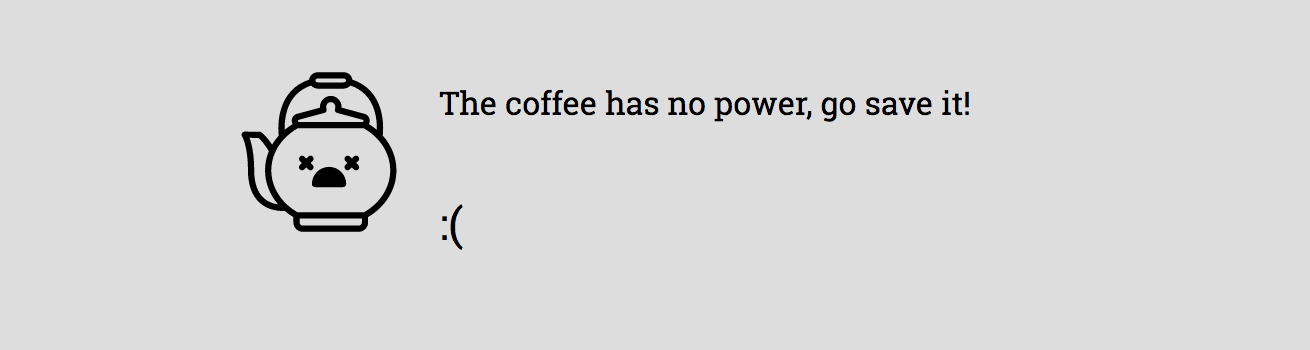
\includegraphics[width=0.9\textwidth]{figures/nopower}
  }
  \subbottom[When it has been brewing, but at some point lost power for 13 minutes.]{
    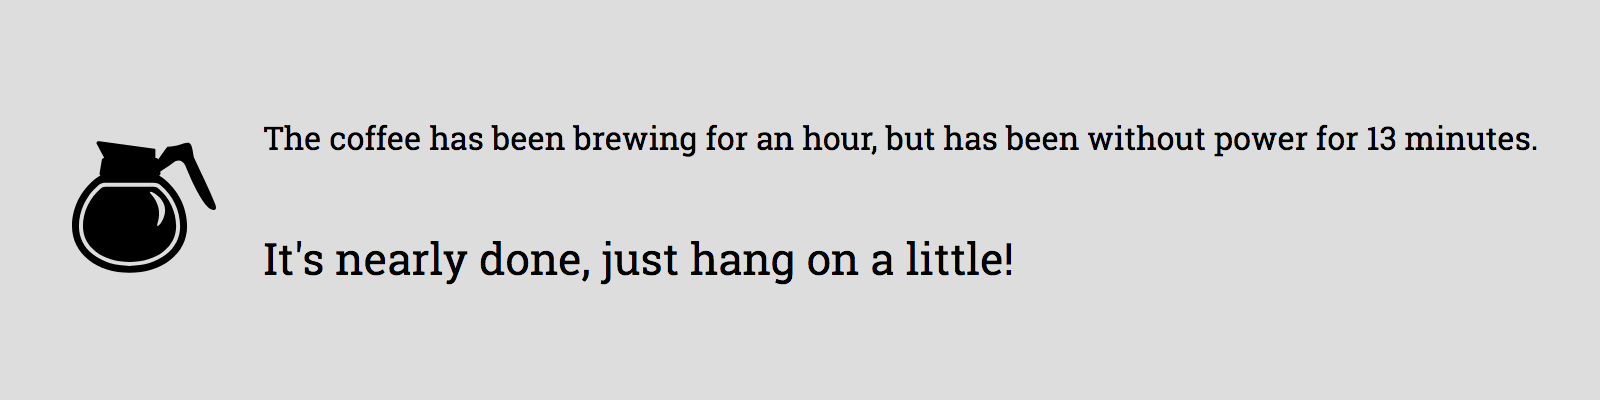
\includegraphics[width=0.9\textwidth]{figures/brewing}
  }
  \caption{Examples of various states of the brew represented on the website.}\label{fig:website}
\end{figure}
The front-end consists of a web application that users can visit in their web
browser and instantly see how the coffee is doing. We decided early on using
React, a JavaScript library for building web application, due to its popularity
as a learning experience. Some examples of the web application be seen in figure
\ref{fig:website}. The web application is in many ways similar to the event loop
in our back-end in that it automatically attempts to fetch the latest data from
the API every 10 seconds.

When a user visits the web application they are presented with an overview page
listing the current state of the coffee. These states are represented by an icon
showing the current amount of coffee or if it is without power and two lines of
flavor text explaining how the brew is doing and whether it is safe to go grab a
cup right now. For example, if the coffee is nearly empty the icon is a coffee
carafe that is nearly empty, and the user is told that ``you better run'' to
emphasize that you need to grab the coffee with due haste. A history page is
also included if the user wants to see the trends for the coffee. This page
lists the last 25 readings of the brewer, allowing the user to at a glance see
how the coffee has been doing for the last few minutes.

\section{Conclusion}\label{sec:conclusion}
We have created a system that successfully monitors the coffee in a drip coffee
brewer. Current and infrared temperature sensors connected to an Arduino gather
information about the age and temperature of the coffee. The temperature and
current is then sent to a Raspberry Pi via an USB serial interface. Using a
camera connected to the Raspberry Pi, we capture images of the coffee pot to
measure the amount of coffee in the container. Processing this data in turn
gives us an insight in the temperature, age, and quantity of the coffee. These
sensor are non-intrusive, as to not discourage the students from brewing and
drinking that sweet coffee. A Django REST API then presents temperature, age and
amount to the outside world enabling others to create their own interface and
representation of what the state of the coffee is. For others we have created a
website to make it accessible for the masses.
 
\section{Future work}\label{sec:future-work}
There are still quite a few features left that we would like to implement and 
others that would-be-cool-to-have. The biggest, and probably most pressing 
item to do is some sort of casing for the hardware. We had grand plans of 
creating a nice 3D-printed case for both the Raspberry Pi and Arduino, but time 
was not on our side before the scheduled deadline. This is something that we 
would like to be able to do during the summer so that it is ready for the new 
students arriving this fall.

The front-end is simple and could benefit from having more pages showing
historical data. The potential for how and what is represented is vast. When 
discussing the project with students while we are testing the system some
suggestions keeps reappearing. The most popular is to add a scanner for 
the student IDs to track how much coffee each student drinks, but also tracking 
who makes the most coffee or who takes the last cup of coffee without making a 
new one. Second most popular is to track how many liters of coffee is 
consumed and being able to extract fun and interesting data from this. For 
example, how much more coffee is consumed during the exam period compared to a 
regular day.

\section{Acknowledgements}\label{sec:acknowledgements}
We would like to thank our supervisor Albin Severinson for giving us helpful, 
and rapid feedback during our almost weekly meetings, as well as Hjalmar 
Svenstrup Andersen and Sondre Vestad for consulting us on the matters of 
electronics and hardware.

\clearpage
\appendix
\chapter{Licenses}\label{sec:licenses}
Both the code in the back-end and front-end are licensed under the MIT License,
a very popular open-source license. The primary reason for choosing this was due
to the very permissive nature of the license, in essence all it requires is
preservation of copyright and license notices. For derivative works you may
freely license them under whatever terms you want and with or without the
aforementioned source code.

The code for the Arduino however required the usage of a library that was
licensed under the APGLv3 license. The family of GPL licenses are what many call
viral licenses, if you use a library in your program that is licensed under
these your program is in essence infected and you now have to license yours
under the same license as well. Hence, this code is licensed under GPL.

\chapter{Parts}\label{sec:parts}
% Fix formating
\begin{itemize}
\item \textbf{Raspberry Pi Camera Module v2.0} \newline
Manufacturer: Raspberry Pi Foundation

\item \textbf{Contact-less Infrared Temperature Sensor} \newline
Manufacturer: Melexis \newline
Part no. MLX90614

\item \textbf{Non-invasive Current Sensor} \newline
Manufacturer: EChun Electronic \newline
Part no. ECS1030-L72

\item \textbf{Raspberry Pi 3 Model B+} \newline
Manufacturer: Raspberry Pi Foundation 

\item \textbf{Arduino Uno Rev3} \newline
Manufacturer: Arduino

\end{itemize}

\chapter{API Reference}\label{sec:api-reference}
Our API is a REST API, a stateless web service for making HTTP requests to
endpoints that return data. In our case you can only ever get data from the API,
it only supports GET requests. Any other kind is rejected by the server,
therefore there are no security concerns with the API as you cannot send data to
it. There are two types of requests a user can do, either they can get the
latest data, or the last 25 data points.

A request to our server with the \lstinline{/api/v1/coffee/now} endpoint would
respond with a JSON object containing the latest reading if the request is valid:

\lstset{
    string=[s]{"}{"},
    stringstyle=\color{blue},
    comment=[l]{:},
    commentstyle=\color{black},
}
\begin{lstlisting}
{
  "id": 223,
  "measured_at": "2019-04-08T17:42:09.723021+02:00",
  "temperature": 45,
  "amount": 0.5,
  "status": 1,
  "brew_started": "2019-04-08T17:33:34.161737+02:00",
  "brew_outages": "00:00:00"
}
\end{lstlisting}

For users who want to consume our API there is generated an automatic API
reference that is available under \lstinline{/swagger/} that documents how to
connect and use them. For more information, the source code for the API is
available at {\small\url{https://github.com/inf219-mocca/MOCCAPI}}.

\clearpage{}
\renewcommand*{\UrlFont}{\footnotesize\ttfamily}
\printbibliography{}

\end{document}
%%% Local Variables:
%%% mode: latex
%%% TeX-master: t
%%% End:
